%%%%%%%%%%%%%%%%%%%%%%%%%%%%%%%%%%%%%%%%%%%%%%%%%%%%%%%%%%%%%%%%%%%%%%%%%%%%%%%

\chapter{CASE STUDY: HURRICANE BERYL}
\label{ch:beryl}

This chapter explores the results of implementing cold pool parameterization in the latest Brazilian numerical weather and climate prediction model, MONAN. It emphasizes the model's performance in predicting hurricane trajectory, intensity, and rainfall, using Hurricane Beryl as a case study, which occurred between June and July 2024 in the North Atlantic Basin. Following a brief introduction to the event, the chapter presents the results of the forecast and offers a direct comparison between ERA5 and MONAN. Finally, a discussion section will address the questions outlined previously in Table \ref{tab:questions}.
% VISTO

\section{Event description - hurricane Beryl}

Hurricane Beryl formed in the deep tropical Atlantic’s Main Development Region on June 28th, forming a tropical depression near 1200 UTC 28 June about 1200 nautical miles \footnote{In North American meteorology, it is common to use: pressure in millibars (mb), where 1 mb = 1 hPa; distance in nautical miles (nm), where 1 nm = 1.852 km; wind speed in knots (kt), where 1 kt = 1.852 km/h; and precipitation in inches (in), where 1 inch = 25.4 mm} east of Barbados, with a center at 1007 mb and wind speed of 30 kts. According to reports from the National Oceanic and Atmospheric Administration (NOAA), the storm rapidly intensified into a major hurricane, moving eastward and ultimately reaching Category 5 on the Saffir-Simpson Hurricane Wind Scale, making it the earliest Category 5 hurricane on record in the Atlantic Basin. Figure \ref{fig:hurricanepath} display all the trajectory computed with the best track dataset.

\begin{figure}[h!]
	\centering
	\caption{2024 Hurricane path according to best track analysis}
	\label{fig:hurricanepath}\includegraphics[width=\textwidth,height=\textheight,keepaspectratio]{docs/figuras/chapter5/beryl_2024.png}
	\centering
	Source: Made by the author (2025).
\end{figure}

It is important to note that the figure presented in the upper-right quadrant indicates critical meteorological parameters, including the peak wind speed recorded at 145 knots, the minimum mean sea level pressure of 934 hPa, and the Accumulated Cyclone Energy (ACE), which is quantified at 34.5. These values are derived directly from the best track dataset.

The first landfall of Hurricane Beryl occurred on the island of Carriacou in Grenada as a high-end Category 4 storm on July 1st, subsequently intensifying to a Category 5 in the Eastern Caribbean Sea. From a disaster perspective, the total damages in the Grenada Region are significant, with estimates of approximately US\$ 218.0 million, which accounts for about 16.5 percent of the GDP for 2023 \cite{gunasekera2024global}. Satellite images illustrating the hurricane's transition from Category 4 to Category 5, passing through the first landfall, are presented in Figure \ref{fig:HurricaneBerylBand13}.

\begin{figure}[h!]
	\centering
	\caption{Hurricane Beryl view from the GEOCOLOR composite (left) and Band 13 (right) when passing through the first landfall}
	
	\begin{minipage}{.48\textwidth}
		\centering
		\includegraphics[width=\linewidth]{docs/figuras/chapter5/20241831150_GOES16-ABI-FL-GEOCOLOR-AL022024-2000x2000.jpg}
		\label{}
	\end{minipage}%
	\hfill
	\begin{minipage}{.48\textwidth}
		\centering
		\includegraphics[width=\linewidth]{docs/figuras/chapter5/20241831710_GOES16-ABI-FL-13-AL022024-2000x2000.jpg}
		\label{fig:HurricaneBerylBand13}
	\end{minipage}
Source: \url{https://www.star.nesdis.noaa.gov/star/index.php.}
\end{figure}

At the passage through the Caribbean region, the rainfall was more intense in Jamaica, with widespread totals between 8 to 12 inches, and a peak of 13.62 inches observed at Knockpatrick in Manchester Parish, representing the highest storm-total rainfall reported.

The storm began to weaken before making a second landfall on the Yucatán Peninsula as a high-end Category 2 hurricane early on July 5th. Following its passage through the Peninsula, the hurricane continued to weaken while moving northwest, influenced by a large mid to upper-level trough of low pressure over the Central U.S., which eroded the robust ridge of high pressure over the Gulf of Mexico \cite{li2025generative}. The combination of increasing wind shear and dry air entrainment maintained a nearly steady state until dawn on July 7th. Later that morning, Hurricane Beryl progressed toward the Central Texas coast (northwest) as the mid to upper-level trough deepened to the north. An influx of moisture and decreased wind shear allowed the storm to become better organized, resulting in it being classified as a Category 1 hurricane by 11 PM CDT on July 7th (04:00 UTC on July 8th). A glimpse of this large scale environment is shown at Figure \ref{fig:mlsp}.

\begin{figure}[h!]
	\centering
	\caption{500 mb Geopotential Height and MSLP at July 8th, 00:00 UTC}
	\label{fig:mlsp}\includegraphics[width=\textwidth,height=\textheight,keepaspectratio]{docs/figuras/chapter5/beryl02l.png}
	\centering
	Source: \url{https://storm.aoml.noaa.gov/viewer/?projectName=BASIN}.
\end{figure}

At approximately 4 AM CDT on July 8th (09:00 UTC on July 8th), the hurricane made landfall near Matagorda along the Texas coast. Its maximum sustained winds were about 129 km/h (80 mph), and its minimum central pressure was 979 hPa. Figure 3 shows satellite and radar imagery capturing Hurricane Beryl's approach to the Texas coast.

\begin{figure}[h!]
	\centering
	\caption{HB view from NEXRAD (top) and GEOCOLOR composite (bottom) when reaching the Texas Coast.}
	\label{fig:nexradgeocolor}
	\includegraphics[width=0.8\textwidth]{docs/figuras/chapter5/20240708-0814Z-HGX.png}
	\vspace{3mm}
	\includegraphics[width=0.6\textwidth]{docs/figuras/chapter5/20241901240_GOES16-ABI-FL-GEOCOLOR-AL022024-2000x2000.jpg}
	
	\centering
	Source: \url{https://www.star.nesdis.noaa.gov/star/index.php.}.
\end{figure}

Finally, the storm began to shift north-northeast, becoming a tropical storm by 10 AM CDT (15:00 UTC on July 8th). As it moved through the continental region, it weakened and transitioned to a tropical depression by 10 PM CDT (03:00 UTC on July 9th), just northwest of Shreveport, Louisiana.

Over the United States, the most intense rainfall occurred in the Houston metropolitan area in southeastern Texas, where widespread totals ranged from 8 to 12 inches, with local maxima of 14.99 inches in Thompsons and 14.88 inches at a HCFCD station in western Houston \cite{li2025generative}.

Based on this overview of the storm, Figure 4 has been created to illustrate the study area of interest, highlighting the significant landfalls made during its progression.

\begin{figure}[h!]
	\centering
	\caption{Spatial Domain of Hurricane Beryl's Development and Trajectory.}
	\label{fig:spatialdomainberyl}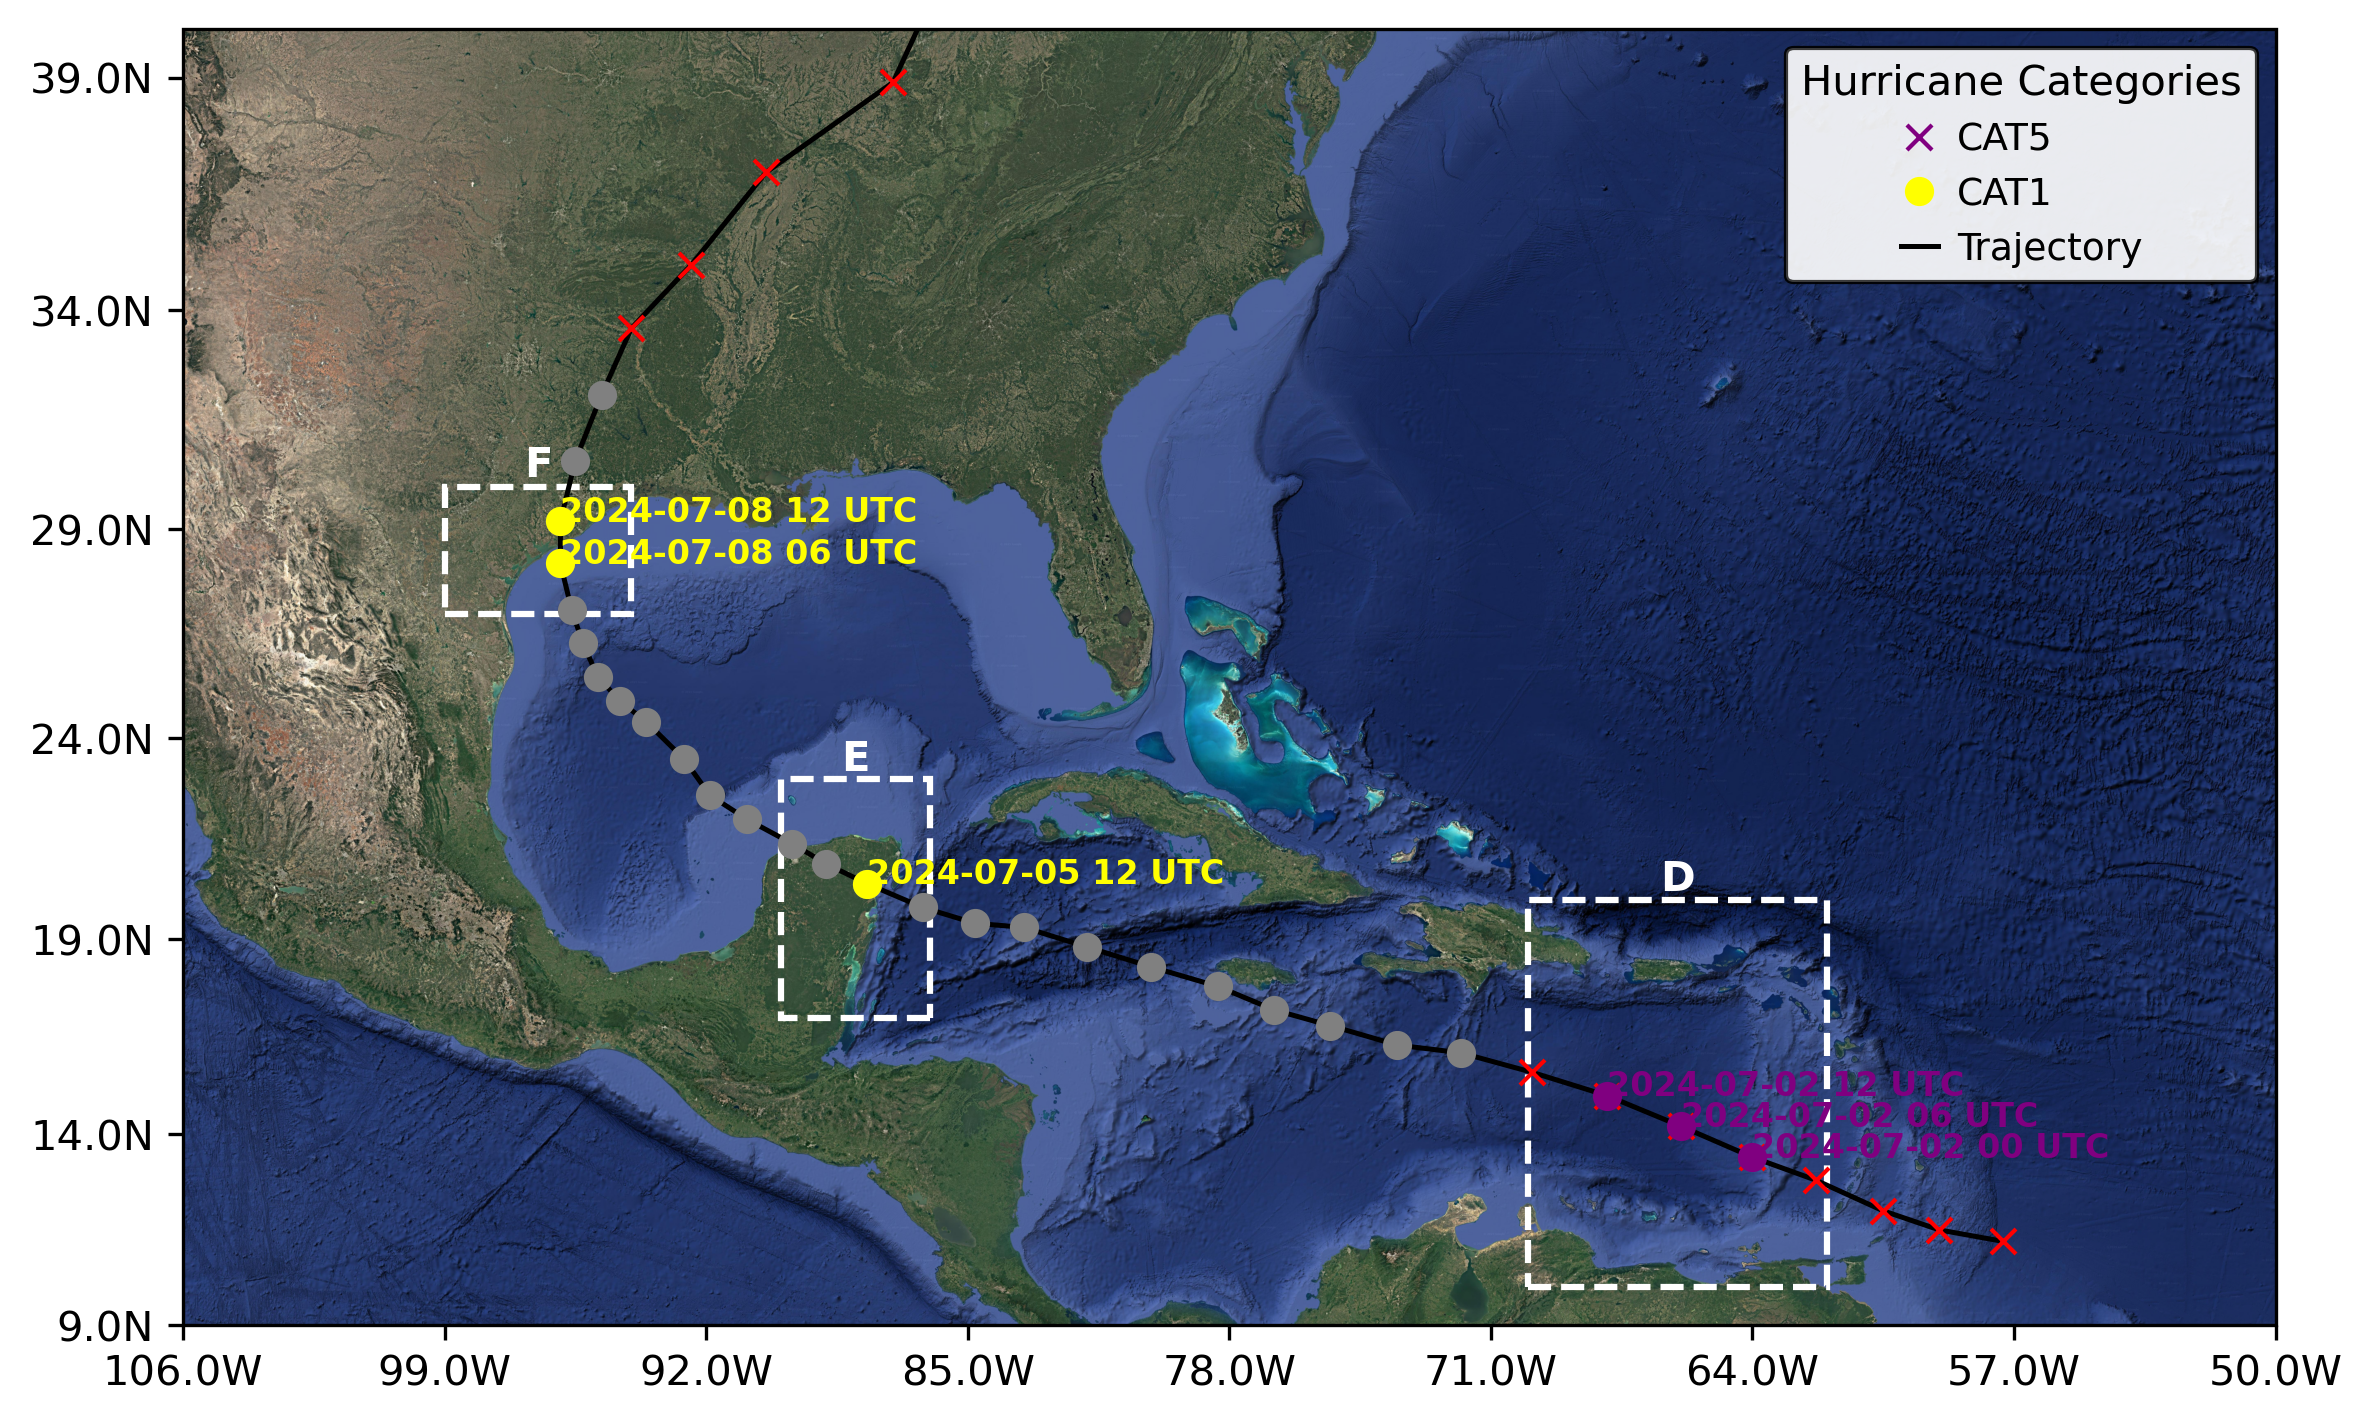
\includegraphics[width=\textwidth,height=\textheight,keepaspectratio]{docs/figuras/chapter5/map_with_cat_path.png}
	\centering
	Source: Made by the author (2025).
\end{figure}

The observational period for this study encompasses a six-day interval from 00 UTC on July 3 to 00 UTC on July 9, 2024, as illustrated by the gray bullet points in Figure \ref{fig:spatialdomainberyl}. Notably, this analysis will focus on a post-Category 5 storm. Whereas the system was active from June 28 to July 9, our analysis concentrates primarily on this specific timeframe. A sensitivity analysis regarding an earlier forecast of the observation period will be conducted and discussed in subsequent sections. This study encompasses significant geographical features, including the passage through Jamaica, which recorded the highest levels of rainfall in the Caribbean, the Yucatan landfall as denoted by the square E in Figure \ref{fig:spatialdomainberyl}, and the subsequent landfall in Texas, indicated by the square F in Figure \ref{fig:spatialdomainberyl}.

% ======================================================================================= %

\section{Results and analysis of hurricane Beryl}

In this section, we will present the results in alignment with the established workflow and engage in a discussion regarding the questions outlined in Table \ref{tab:questions}. The subsequent subsections will detail the trajectory, intensity, and rainfall analyses. To conclude, we will provide a summary discussion highlighting the key outcomes of the model and evaluating the overall performance of MONAN in comparison with ERA5 reanalysis.

By the workflow sequence, we will begin by addressing the selection process. Table~\ref{tab:experiments_long} illustrates all the experiments that were conducted.

\begin{table}[H]
	\centering
	\caption{All performed experiments}
	\label{tab:experiments_long}
	\renewcommand{\arraystretch}{1.2}
	\resizebox{\textwidth}{!}{
		\begin{tabular}{
				>{\centering\arraybackslash}m{3.5cm}
				>{\centering\arraybackslash}m{9cm}
				>{\centering\arraybackslash}m{4cm}
			}
			\toprule
			\textbf{Experiment} & \textbf{Description} & \textbf{ID} \\
			\midrule
			
			Cold Pool Effect 
			& Turn on and off the cold pool parameterization scheme 
			& \makecell[l]{CP-ON\\CP-OFF (Control)} \\
			\midrule
			
			Initial Condition Day 
			& Compares the effect of two initial conditions, June 29, July 2nd (noon), and July 3rd. Tested with 1st July 
			& \makecell[l]{CP-29\\CP-01\\CP-02T12\\CP-03} \\
			\midrule
			
			Cold Pool Lifetime 
			& Compares the effect of cold pool life time being 1h, 2h (default), 3h, and 6h 
			& \makecell[l]{CP-1H\\CP-2H\\CP-3H\\CP-6H} \\
			\midrule
			
			Maximum Downdraft Height 
			& Compares the effect of the maximum downdraft height, being 0.25, 0.35, and 0.50 
			& \makecell[l]{CP-D025\\CP-D035\\CP-D050} \\
			\midrule
			
			Resolution Experiment 
			& Evaluate the resolution effect on the results, degrading it into 60 km and enhancing it into 15 km 
			& \makecell[l]{CP-15km\\CP-30km (Control)\\CP-60km} \\
			\midrule
			
			Type of Initial Condition 
			& Changes the type of initial condition to be from the GFS model 
			& \makecell[l]{CP-ERA5 (Control) \\(CP-GFS)} \\
			\midrule
			
			Best Configuration Test 
			& A run with 2 changes inside the cold pool parameters 
			& \makecell[l]{CP-1HD050\\CP-1HD05015km} \\
			\bottomrule
		\end{tabular}
	}
	
	\vspace{2mm}
	{\centering Source: Made by the author (2025).\par}
\end{table}

The “ID” column serves as a reference for the names of the experiments. It is important to note that in the results, CP-ON represents the default configuration. In the sensitivity analyses conducted, the default values are specified in the labels. For instance, in the “Resolution Experiment,” the default configuration is set to a grid of 30 km (CP-30km), which is then changed to 60 km (CP-60km) and 15 km (CP-15km). To clarify, the following table emphasizes the default parameters:

\begin{table}[H]
	\centering
	\caption{Default values for the cold pool parameterization scheme}
	\label{tab:cp_def}
	\renewcommand{\arraystretch}{1.2}
	\resizebox{\textwidth}{!}{
		\begin{tabular}{
				>{\centering\arraybackslash}m{5.5cm} 
				>{\centering\arraybackslash}m{9cm}
			}
			\toprule
			\textbf{Parameter} & \textbf{Default value} \\
			\midrule
			Initial Condition Day & July 3rd, 2024 \\
			Cold Pool Lifetime & 2 h \\
			Maximum Downdraft Height & 0.35 \\
			Resolution Experiment & 30 km horizontal grid \\
			Type of initial condition & Coming from ERA5 \\
			\bottomrule
		\end{tabular}
	}
	
	\vspace{2mm}
	{\centering Source: Made by the author (2025).\par}
\end{table}




We investigate the impact of cold pools by enabling (CP-ON) and disabling (CP-OFF) the parameterization, with CP-OFF serving as the control experiment in this case. In the subsequent rows, we conducted a sensitivity analysis on the parameters within the parameterization. Now our control experiment is the CP-ON configuration, with the Table \ref{tab:cp_def} parameters. For the “Initial Condition Day” experiment, we varied the initial integration times: June 29 (00 UTC), 2024; July 1 (00 UTC), 2024; and July 2 (12 UTC), 2024 - comparing them with the default time. These periods were selected because they correspond to key moments in the storm’s evolution: shortly after HB was classified as a tropical storm, one day before it reached Category 5, and the day it reached Category 5, respectively.

The “Cold Pool Lifetime” was adjusted from the default to durations of 1 hour, 3 hours, and 6 hours. The height of the mass flux above the surface is described by a parabolic function, and the coefficient of this function can be manipulated to alter the maximum height, with lower (higher) values indicating proximity (distance) to the surface. The “Type of Initial Condition” was switched from ERA5 to GFS, both initialized on July 3 (00 UTC), 2024.

During the computation of the initial 13 experiments, we observed that setting the cold pool lifetime to 1 hour and adjusting the maximum downdraft height coefficient to 0.5 resulted in lower errors in the initial results. Consequently, we conducted the “Best Configuration Test” with these parameter adjustments and repeated this configuration at 15 km, bringing the total number of experiments to 15. The reference data here is the best track dataset, and hereafter this dataset will be referenced as “NOAA”. 

Keeping this in mind, Figure~\ref{fig:all_tracks_before} shows all the trajectories for the 15 experiments, plus ERA5 and the reference best-track dataset.

\begin{figure}[!htb]
    \centering
    \caption{Comparison of Storm Tracks Across All 15 Experiments} % Título acima da figura
    \includegraphics[width=\textwidth]{docs/figuras/chapter5/ALL_tracks_before_filter.png} % Substitua pelo caminho e extensão correta
    \vspace{0.5em}
    
    Source: Made by the author (2025). % Fonte abaixo da imagem
    \label{fig:all_tracks_before} % Label para referenciar no texto
\end{figure}

As one can see in Figure~\ref{fig:all_tracks_before}, the numerous experiments clutter the scene and make visual comparison difficult. But one could notice the deviation of CP-6H and CP-01, which could be candidates to be withdrawn. To better visualize the difference between the trajectories, the distance between each trajectory and the reference data (NOAA’s best track) was computed and shown in Figure~\ref{fig:panel_errors_before}.

\begin{figure}[!htb]
    \centering
    \caption{Errors (distance) between the trajectories} % Título acima da figura
    \includegraphics[width=\textwidth]{docs/figuras/chapter5/panel_2x2_error_comparison.png} % Substitua pelo caminho e extensão correta
    \vspace{0.5em}
    
    Source: Made by the author (2025). % Fonte abaixo da imagem
    \label{fig:panel_errors_before} % Label para referenciar no texto
\end{figure}

\pagebreak

It can be confirmed that CP-01 deviates significantly from the expected trajectory. Additionally, CP-6H offer limited discussion, as it is quite similar to the other experiments within their group. In Figure~\ref{fig:panel_errors_before} (d), CP-1HD05015km does not show a significant improvement and will consequently be withdrawn. We will retain CP-1HD050 to seek the effects related to this configuration in the context of other aspects of tropical cyclones.

To summarize the experiments we intend to keep, a new table has been created, similar to Table~\ref{tab:experiments_long}.

\pagebreak

\begin{table}[H]
	\centering
	\caption{Selected experiments}
	\label{tab:selected_experiments}
	\renewcommand{\arraystretch}{1.2}
	\resizebox{\textwidth}{!}{
		\begin{tabular}{
				>{\centering\arraybackslash}m{4cm}
				>{\centering\arraybackslash}m{9cm}
				>{\centering\arraybackslash}m{4cm}
			}
			\toprule
			Parameter & Description & ID \\
			\midrule
			
			Cold Pool Effect 
			& Turn on and off the cold pool parameterization scheme 
			& \makecell[l]{CP-ON\\CP-OFF (Control)} \\
			\midrule
			
			Initial Condition 
			& Compares the effect of two initial conditions, June 29, July 2nd (noon), and July 3rd. Tested with 1st July 
			& \makecell[l]{CP-29\\CP-02T12\\CP-03 (Control)} \\
			\midrule
			
			Cold Pool Lifetime 
			& Compares the effect of cold pool life time being 1h, 2h (default), 3h, and 6h 
			& \makecell[l]{CP-1H\\CP-2H (Control)\\CP-3H} \\
			\midrule
			
			Maximum Downdraft Height 
			& Compares the effect of the maximum downdraft height, being 0.25, 0.35, and 0.50 
			& \makecell[l]{CP-D025\\CP-D035 (Control)\\CP-D050} \\
			\midrule
			
			Resolution Experiment 
			& Evaluate the resolution effect on the results, degrading it into 60 km and enhancing it into 15 km 
			& \makecell[l]{CP-15km\\CP-30km (Control)\\CP-60km} \\
			\midrule
			
			Type of Initial Condition 
			& Changes the type of initial condition to be from the GFS model 
			& \makecell[l]{CP-ERA5 (Control)\\(CP-GFS)} \\
			\midrule
			
			Best Configuration Test 
			& A run with 2 changes inside the cold pool parameters 
			& CP-1HD050 \\
			\bottomrule
		\end{tabular}
	}
	
	\vspace{2mm}
	{\centering Source: Made by the author (2025).\par}
\end{table}


In the following subsection we will continue the results now keeping in mind the experiments listed at Table~\ref{tab:selected_experiments}.

%%%%%%%%%%%%%%%%%%%%%%%%%%%%%%%%%%%%%%%%%%

\subsection{Trajectory}


All trajectories are displayed in the Figure~\ref{fig:all_tracks_selected}. The trajectories of each group of the Table~\ref{tab:selected_experiments} can be found at Appendix B.

\begin{figure}[!ht]
    \centering
    \caption{All tracks with selected experiments from Table~\ref{tab:selected_experiments}} % Título acima da figura
    \includegraphics[width=\textwidth]{docs/figuras/chapter5/ALL_tracks_filter.png} 
    \vspace{0.5em}
    
    Source: Made by the author (2025). % Fonte abaixo da imagem
    \label{fig:all_tracks_selected} % Label para referenciar no texto
\end{figure}

This figure presents a map generated utilizing a tracking algorithm developed by the author. Firstly, the algorithm extracts each point corresponding to the minimum central pressure from the best track data between July 3rd and July 9th, 2024, sweeping a total integration period of 144 hours, with data plotted at 6-hour intervals. Furthermore, the minimum Mean Sea Level Pressure (MSLP) of the MONAN’s forecast and ERA5 reanalysis is extracted within a predefined spatial box surrounding the best track minimum central pressure. For instance, the initial bullet point depicted in dark green (representing NOAA’s best track at approximately 72.5° W) corresponds to the minimum central pressure obtained with the best track on July 3rd (00 UTC), 2024, while the final bullet point in dark green represents the data from July 9th (00 UTC), 2024 (close to 95° W).

At first glance, the reader will notice the observed congruence between the ERA5 reanalysis data and the best track observations. This strong agreement may be attributable to the reanalysis nature (Dulac et al., 2023), which integrates observational datasets throughout the integration period, thereby leading to this expected behaviour.

The CP-ON and CP-OFF experimental configurations exhibit comparable results for the majority of the integration period, with pronounced discrepancies evident near the Texas landfall and around the Yucatán Peninsula. A more detailed examination of these differences is warranted with other metrics. Concerning the cold pool lifetime, a 3-hour interval significantly deteriorates the accuracy of the forecasts. Furthermore, the downdraft maximum height coefficient of 0.50 appears to yield less precise results relative to the default values of 0.35 and 0.25. The trajectory forecasts utilizing a 60 km horizontal resolution demonstrate closer alignment with the reference data, outperforming the 15 km and 30 km horizontal resolutions, with the 60 km configuration exhibiting superior performance. Additionally, forecasts initialized with the GFS (CP-GFS) model appear to underperform in comparison to those initialized with ERA5.

It is observed that when initialization occurs before July 3rd (00 UTC), 2024, a visible degradation in trajectory forecast accuracy ensues. Note that there is a tendency for earlier initialization to result in poorer forecasts, a fact that can be confirmed later on with the MAE and RMSE metrics. This underscores the necessity of incorporating a module within the model to assess ensembles of initial conditions, also in agreement with what is found in the literature \cite{donkin2023capability}.

Finally, the configuration incorporating two parameters that have been changed simultaneously does not reveal significant deviations from the default setup. Overall, the forecasts exhibit a westward bias, a phenomenon that is also apparent in forecasts issued by the Hurricane Analysis and Forecast System (HAFS), as shown at Figure \ref{fig:berryl3rd}.

\begin{figure}[!ht]
	\centering
	\caption{Forecast made for Hurricane Beryl starting at July 3rd (00 UTC), 2024, available at the HAFS website} % Título acima da figura
	\includegraphics[width=\textwidth]{docs/figuras/chapter5/HAFS_trajectory.png} 
	\vspace{0.5em}
	Source: \url{https://www.emc.ncep.noaa.gov/HAFS/HAFSEPS/index.php} . % Fonte abaixo da imagem
	\label{fig:berryl3rd} % Label para referenciar no texto
\end{figure}

The next panel provides complementary information to the analysis, now in a more quantitative manner. It is important to mention that the time series display the errors after 12h of spin-up, and that value is maintained and the further analysis. In Figure (a), it is possible to better distinguish the differences among the experiments over time. In other words, it shows when each experiment presents lower errors throughout the integration period, along with an initial comparison among them. It is important to note that the vertical line E indicates the moment the hurricane makes landfall on the Yucatan Peninsula, while the vertical line F marks its entry into Texas. In Figure (b), this comparison becomes even clearer, especially because the bars are arranged vertically from the lowest to the highest error (from top to bottom).

\begin{figure}[!ht]
	\centering
	\caption{Track errors of the MONAN forecast and ERA5 reanalysis with the best track as reference. 12 hours of model spin-up are withdrawn from the analysis. (a) is displayed the distance error computed as the great circle, and (b), the MAE and RMSE calculated from (a).} % Título acima da figura
	\includegraphics[width=\textwidth]{docs/figuras/chapter5/panel_errors_mae_rmse_FINAL.png} 
	\vspace{0.5em}
	Source: Made by the author, (2025).  % Fonte abaixo da imagem
	\label{fig:trackerrors} % Label para referenciar no texto
\end{figure}

As shown in the previous figure, ERA5 delivers the best track prediction performance. This could be attributed to the fact that ERA5 is a reanalysis product, meaning that observational data assimilation is injected into the model at each integration step. A fairer comparison would require conducting this analysis with another model similar to MONAN, which will be left for future work.

Overall, forecasts tend to show errors below 100 km up to 42 hours of lead time, except for those initialized earlier (CP-29 and CP-02T12). After 60 hours of forecast (two and a half days), some experiments begin to exceed 200 km of error. However, cold pool influence on track prediction only reaches this threshold after 84 hours (three and a half days), and the CP-D025 experiment only reaches it after about 111 hours (four and a half days). Therefore, we observe that with cold pool parameterization, forecast skill is extended by up to two days compared to the configuration without this scheme, for this specific case study.

In the literature, the best forecast limit reported is around 120 hours (five days) \cite{zhou2020prospects}, \cite{sippel2022impacts}. It is worth emphasizing that forecast errors beyond this threshold should be considered “chaotic,” given the nonlinear nature of the system.

The computation of MAE and RMSE provides insights into the overall error behavior in track forecasts. While MAE offers a generalized view of the error, RMSE takes into account the squared deviations, assigning more weight to larger errors at each time step. In general, it is notable that simply enabling the cold pool parameterization (CP-ON) already improved the track forecast, reducing the MAE by approximately 22\% compared to CP-OFF. Furthermore, we observe that tuning the parameters, such as in CP-D025, CP-3H, and modifying the resolution to 60 km (CP-60km), further enhanced this performance.

By observing the Figure \ref{fig:berryl3rd} and Figure \ref{fig:trackerrors}, one could notice the westward deviation in the forecast. The next panel showing the CTE and ATE can confirm this behaviour, at Figure \ref{fig:cte}.

\begin{figure}[!ht]
	\centering
	\caption{CTE (a) and ATE (b).} % Título acima da figura
	\includegraphics[width=\textwidth]{docs/figuras/chapter5/Cross_Track_Along_Track_Errors_FINAL.png} 
	\vspace{0.5em}
	Source: Made by the author, (2025).  % Fonte abaixo da imagem
	\label{fig:cte} % Label para referenciar no texto
\end{figure}

Overall, most of the forecasts show a negative CTE, meaning there is a leftward (westward) deviation from the observed trajectory, confirming Figure \ref{fig:all_tracks_selected}, which displays all the tracks, and Figure \ref{fig:berryl3rd}. This trend is particularly clear in the CP-02T12 experiment. Since the first hour of the forecast, the CTE is negative, which aligns with the fact that the predicted trajectory is consistently to the left of the observed one.

It is interesting to note that the CTE behavior differs significantly between the CP-ON and CP-OFF experiments. While CP-OFF maintains a positive CTE, CP-ON gradually shifts to a negative CTE as the integration period progresses. Notably, CP-ON begins to deviate leftward after around 72 hours of integration, after passing through the Yucatan Peninsula, whereas in other experiments, such as CP-OFF and CP-D025, this deviation occurs earlier.

Interestingly, despite exhibiting large overall errors (Figure \ref{fig:trackerrors}), the CP-D050 experiment performs better than CP-ON in this metric, as it does not deviate as strongly. This highlights the importance of evaluating forecast performance from multiple perspectives and understanding the sources of these differences, which we will further investigate using meteorological fields.

This westward bias was also noted in the forecasts from both the HAFS (Figure \ref{fig:berryl3rd}) and the UK Met Office  (Figure \ref{fig:metoff}) for Hurricane Beryl.

\begin{figure}[!ht]
	\centering
	\caption{Tracking available by the UK Met Office.} % Título acima da figura
	\includegraphics[width=\textwidth]{docs/figuras/chapter5/MetOffice.png} 
	\vspace{0.5em}
	Source: \url{https://www.metoffice.gov.uk/research/weather/tropical-cyclones/verification/seasons/nhem2024.}  % Fonte abaixo da imagem
	\label{fig:metoff} % Label para referenciar no texto
\end{figure}

The report \cite{metoffice2024} indicates that the track was forecasted with a notable degree of accuracy throughout the Caribbean region, furthermore, it was observed that there was a left-of-track bias in the forecasts as Beryl progressed into the Gulf of Mexico.

In general, the ATE is positive across all experiments, indicating a consistent tendency for the MONAN model to move faster than observed. Note that ERA5 also displays this trend, though it is not as pronounced as in MONAN.

When comparing CP-ON and CP-OFF, a growing ATE trend is evident in CP-OFF. As the integration period increases, CP-OFF moves increasingly ahead of the observed track, reaching 225 km ahead at 66 hours, whereas CP-ON is only about 150 km ahead at the same time.

The CP-D025 experiment appears to be more in phase with the observations in this metric than CP-ON during most of the forecast period, despite having a greater leftward deviation compared to CP-ON. Despite larger errors in track positioning, the early-initialized forecasts manage to better match the best track in terms of propagation speed. In this case, the forecast initialized with GFS outperformed the forecast initialized with ERA5 during most of the integration period.

A mean error performance of all MONAN forecasts were computed and shown at Figure \ref{fig:monera5}.

\begin{figure}[!ht]
	\centering
	\caption{Overall performance of MONAN trajectory forecasts compared with ERA5 reanalysis.} % Título acima da figura
	\includegraphics[width=\textwidth]{docs/figuras/chapter5/barplot_monan_vs_era5_mae_rmse_FINAL.png} 
	\vspace{0.5em}
	Source: Made by the author (2025).  % Fonte abaixo da imagem
	\label{fig:monera5} % Label para referenciar no texto
\end{figure}

In general, the MONAN forecast is approximately 8 times greater than the ERA5 reanalysis. Again, we can infer that it is not a fair comparison between the MONAN forecast and the ERA5 reanalysis, but it is important to notice the error scale to give us insights about improving the MONAN forecast.



\subsection{Intensity}

The minimum MSLP found in the track and best track was plotted as Central Pressure in Figure \ref{fig:monera5} (a). The forecasted wind at the first model level alongside with the maximum wind speed of best track and the 10 meters instantaneous gust-front of ERA5 are displayed in Figure \ref{fig:monera5} (b). The Saffir-Simpson wind scale is denoted by black lines to guide the reader in the forecast scale. 

\begin{figure}[!ht]
	\centering
	\caption{Comparison of Forecasted and Observed Central Pressure and Wind Speeds for Hurricane Beryl. Here, a 12-hour model spin-up was also withdrawn, starting the time series on July 3rd, 12 UTC.} % Título acima da figura
	\includegraphics[width=\textwidth]{docs/figuras/chapter5/intensity_time_series_panel_FINAL.png} 
	\vspace{0.5em}
	Source: Made by the author (2025).  % Fonte abaixo da imagem
	\label{fig:monera5} % Label para referenciar no texto
\end{figure}

In general, this panel indicates that the ERA5 reanalysis demonstrates poorer performance in predicting central pressure compared to MONAN forecasts. This finding aligns with the work of \citeonline{dulac2024assessing}, who highlight that inaccuracies in central pressure estimations can lead to underestimations in wind speed intensity predictions. Given that MONAN is initialized with ERA5 reanalysis fields, it is anticipated that the initial conditions also carry those uncertainties.

As shown in Figure \ref{fig:monera5} (a), the MONAN forecasts exhibit a similar trend; however, there are notable outliers, particularly in the CP-29 and CP-02T12 experiments, especially following the Texas entrance (marked by the vertical line "F").

The initial high-pressure peak occurring between 24 and 30 hours of the forecast is in phase with the best track. However, after the passage of the Yucatan Peninsula, at 66-72 hours of forecast, the experiments fall out of phase by approximately 6 hours, with MONAN displaying an earlier peak than the best track. A forecasted low-pressure system intensifies around 102-108 hours, while the best track identifies this feature closer to 126 hours. This behavior is consistent with what the ATE indicated earlier.

The cold pool effect is most noticeable in Figure \ref{fig:monera5} (b). The CP-ON configuration tends to generate more wind than CP-OFF, yet it does not reach the strength reported in the best track data.

The forecasts initialized earlier than the standard (CP-29 and CP-02T12) in Figure \ref{fig:monera5}  (b) also emerge as outliers. This discrepancy becomes particularly evident when we examine the last intensification moment from the best track, at 120 hours, achieving Category 1. In contrast, these forecasts peak at 90 hours, showing even greater intensity as they reach Categories 2 and 3. This indicates a significant divergence of a full day between these forecasts and the intensity described by the best track. This trend, consistent with the observations in the ATE, is also reflected in the other forecasts. Furthermore, the anticipation of peak intensity worsens as the integration time extends.

One of the most striking forecasts in this figure is from the CP-D025 experiment, which illustrates an excessively intense system. This intensity arises because the mass flux is situated much closer to the surface compared to the other experiments, resulting in stronger downdrafts and, consequently, a more intense gust.

The panel presents a quantitative evaluation of the forecasts and ERA5 reanalysis in comparison to the intensity observed in the best track. The RMSE in these figures is a particularly insightful metric due to the oscillatory nature of the event, as this error is computed as a weighted average of the squared differences.

\begin{figure}[!ht]
	\centering
	\caption{Central Pressure and Maximum Wind Speed Errors.} % Título acima da figura
	\includegraphics[width=\textwidth]{docs/figuras/chapter5/panel_mae_rmse_mslp_wspd_FINAL.png} 
	\vspace{0.5em}
	Source: Made by the author (2025).  % Fonte abaixo da imagem
	\label{fig:errors} % Label para referenciar no texto
\end{figure}

In Figure \ref{fig:errors} (a), the performance of the cold pools in the pressure field is evident, with CP-ON showing a reduction in MAE of approximately 8\% compared to CP-OFF. Furthermore, the importance of investigating and tuning the parameters within this parametrization is highlighted, as modifying them leads to further improvements in pressure representation. Notably, the CP-1HD050 configuration stands out, despite not achieving the same improvement in the wind field. This relationship between cold pools and the pressure field could be further explored in future studies.

In Figure \ref{fig:errors} (b), it is interesting to note that CP-ON reduces the MAE by approximately 12.5\% compared to CP-OFF, while the RMSE shows an even greater reduction of about 20\%. Although the CP-D025 experiment produces a system that is too intense, diverging from the best track, as shown in the previous figure, it does not result in a worsening of the pressure field, once again underscoring the importance of parameter tuning within the convection scheme.

By the end, a mean of Figure \ref{fig:errorsmona} is presented next, to highlight the differences between ERA5 and MONAN.

\begin{figure}[!ht]
	\centering
	\caption{Central Pressure and Maximum Wind Speed errors by MONAN compared to ERA5.} % Título acima da figura
	\includegraphics[width=\textwidth]{docs/figuras/chapter5/barplot_mean_error_monan_era5_intensity_FINAL.png} 
	\vspace{0.5em}
	Source: Made by the author (2025).  % Fonte abaixo da imagem
	\label{fig:errorsmona} % Label para referenciar no texto
\end{figure}

In contrast to the trajectory analysis, the advancements in the forecasting capabilities of MONAN are evident, particularly in the substantial reduction of maximum wind speed, which has decreased by approximately 54\% when compared to the ERA5 reanalysis.














\subsection{Rainfall}

In this subsection, we will analyze the rainfall through three perspectives: the rainfall pattern and spatial distribution; the mean and distribution of rain volume; and the extreme values.

\subsubsection{Pattern and spatial rainfall distribution}

Following the workflow proposed in the Metrics section, we can quantify the spatial distribution of rainfall using the ETS and Pearson correlation coefficient. This analysis focuses on a specific area (106-51°W, 10-41°N) over a six-day forecast period, from July 3rd to July 9th (00 UTC). Upon reviewing the literature \cite{marchok2007validation}, \cite{brackins2020evaluation}, \cite{luitel2018verification}, we found that these metrics are influenced by the forecasted track and are typically calculated over a defined region, usually a 500-600 km radius around the best track trajectory, rather than the broader area we are examining. In their 2007 study, Marchok et al. discuss this in detail and suggest potential improvements to compute those metrics, also regarding resolution dependencies. We opted to calculate the accumulated area to reduce the track error effect, though it is important to note that this approach may also capture local rainfall accumulations. In our study area, identifying the hurricane is relatively straightforward; for example, reports indicate that Beryl produced 13.2 inches (approximately 335 mm) of accumulated rainfall over Jamaica \cite{li2025generative}, so because of this, the broader area should not be this much of a problem, but meant to be a simple view of the spatial rainfall distribution. For future work, we propose adapting the previous approach to more accurately represent both the ETS and Pearson correlation coefficients.

Figure \ref{fig:threatscore} illustrates the ETS for various rainfall thresholds (in mm). These thresholds were determined using a log distribution, similar to the method presented by Marchok et al. in 2007. The maximum threshold was established with consideration of the maximum distribution observed in the datasets \footnote{The Python function used was: \texttt{numpy.logspace(numpy.log10(0.01), numpy.log10(350), num=12)}}. For instance, the maximum accumulated rainfall measured was 252.5 mm, 252.0 mm, 453.7 mm, 485.4 mm, 359.6 mm for GPM-IMERG, ERA5, GSMaP, CP-ON, CP-OFF, respectively.

\begin{figure}[!ht]
	\centering
	\caption{Equitable Threat Score for all experiments, ERA5 dataset and GSMaP dataset.} % Título acima da figura
	\includegraphics[width=\textwidth]{docs/figuras/chapter5/ets_all_experiments_logx_FINAL.png} 
	\vspace{0.5em}
	Source: Made by the author (2025).  % Fonte abaixo da imagem
	\label{fig:threatscore} % Label para referenciar no texto
\end{figure}

The GSMaP exhibits the best score due to its nature as a satellite-based system. It is important to highlight that for this and other analyses, both GSMaP, ERA5, and GPM-IMERG data were downscaled to the model's resolution of 30 km. In the case of GSMaP, the resolution was reduced from 4 km to 30 km. The further analysis will explicitly mention this whenever the data is not downscaled.

ERA5 shows better agreement in the moderate to extreme rainfall range (between 3 and 135 mm), but it is important to note that the maximum rainfall is relatively low compared to GPM-IMERG. Thus, ERA5 does not score well regarding rainfall data produced by this event.

In general, the forecasts from MONAN display similar behavior, with some outliers. For example, CP-OFF shows a better score at the lower thresholds compared to other forecasts, meaning that local rainfall is slightly better in agreement with the observed data, but it displays the same trend in the extreme thresholds. Another outlier is CP-29, which exhibits poor agreement with the observed data, especially due to a poor predicted trajectory.

At more extreme thresholds (above 135 mm), the scores for all data types drop significantly, indicating the need for further investigation into this topic.

The Pearson correlation coefficient is shown next, in Figure XXX. This coefficient was calculated across the entirety of the spatial domain, indicating that it provides a correlation value representative of the entire scene.

\begin{figure}[!ht]
	\centering
	\caption{Spatially averaged Pearson correlation coefficient over the entire domain} % Título acima da figura
	\includegraphics[width=\textwidth]{docs/figuras/chapter5/pearson_correlation_bar_chart_FINAL.png} 
	\vspace{0.5em}
	Source: Made by the author (2025).  % Fonte abaixo da imagem
	\label{fig:pearson} % Label para referenciar no texto
\end{figure}

Once again, the data from GSMaP and ERA5 stand out with the strongest correlations with GPM-IMERG. Interestingly, this highlights the effects that changes in resolution can have, as seen more clearly in the panel of Figure \ref{fig:dpearson}.

Regarding the forecasts from MONAN, the average correlation is around moderate, excluding outliers such as GFS, CP-29, and CP-02T12. Note that for the last two forecasts, the bias from the trajectory itself strongly influences the calculation of this metric, as CP-29 and CP-02T12 also had the largest tracking errors (Figure \ref{fig:trackerrors}).

To better infer the locations with the best/worst correlations, as well as to gain a clearer understanding of the temporal evolution of correlation in the forecasts, Figure \ref{fig:dpearson} displays the correlation spatially, computed from daily rainfall accumulations.

\begin{figure}[!ht]
	\centering
	\caption{Spatial distribution of daily Pearson correlation values to assess temporal evolution of forecast performance} % Título acima da figura
	\includegraphics[width=\textwidth]{docs/figuras/chapter5/painel_correlation_selected_experiments_days_nomeado.png} 
	\vspace{0.5em}
	Source: Made by the author (2025).  % Fonte abaixo da imagem
	\label{fig:dpearson} % Label para referenciar no texto
\end{figure}

In this figure, the selected days represent: (a) the starting point of forecasts, immediately following the weakening of Hurricane Beryl, but corresponding to the highest observed rainfall (over Jamaica); (b) its passage over the Yucatán Peninsula, during which the hurricane weakens from Category 1 to a tropical storm; and (c) landfall in Texas on the North American continent. It is important to note that each column represents the accumulated rainfall for 24 hours; thus, panel (a) corresponds to rainfall accumulated over July 3rd, and so on.

The top row presents correlation values derived from ERA5 reanalysis, which exhibited strong correlations, while the bottom row shows the correlation from the CP-29 forecast, which had the weakest agreement. To evaluate the effect of cold pool parameterization, CP-ON and CP-OFF are aligned for comparison. Additionally, CP-D050 was selected as an example of moderate correlation to identify where the internal parameterization settings are influencing correlation variability. Other experiments referenced in the study are presented in the appendix.

Regarding the temporal evolution of correlation, a general degradation in forecast performance over time is observed, with the reanalysis data maintaining higher consistency, as expected. Notably, CP-29 shows a significantly sharper decline in correlation over time compared to CP-ON, for instance. 

For instance, CP-29 reveals a pronounced track error upon landfall in Texas (100–90°W, 25–35°N), as evidenced by a near-zero correlation in that region. In the same region, CP-D050 and CP-OFF present negative correlations when compared with CP-ON.

CP-D050 fails to represent rainfall over the Yucatán Peninsula, whereas CP-ON appears to generate more cohesive rainfall patterns than CP-OFF (20–25°N, 90–80°W). Both CP-D050, CP-ON, and CP-OFF also show localized overestimation of rainfall east of Cuba, a region that does show rainfall in the ERA5 dataset.

Selected snapshots corresponding to these dates were chosen to confirm the previously discussed relationships. A panel displaying these time steps alongside IMERG and GSMaP (both downscaled to 30 km resolution) is presented in Figure \ref{fig:snapshot}.

\begin{figure}[!ht]
	\centering
	\caption{Selected snapshots of rainfall fields from IMERG and GSMaP (30 km resolution) for key time steps} % Título acima da figura
	\includegraphics[width=\textwidth]{docs/figuras/chapter5/painel_instantaneous_rainfall_selected_with_stats_FINAL.png} 
	\vspace{0.5em}
	Source: Made by the author (2025).  % Fonte abaixo da imagem
	\label{fig:snapshot} % Label para referenciar no texto
\end{figure}

One of the most notable aspects across the panels is the skill of the parameterizations in generating cohesive rainfall patterns (e.g., CP-ON and CP-GFS in column a), and in some cases, reproducing the hurricane's spiral structure (panel b—seen in CP-ON, CP-D050, and CP-GFS).

Regarding maximum and average rainfall, the forecasts tend to overestimate precipitation relative to observations. However, in column (b), both CP-ON and CP-D050 are close to approximating the rainfall amounts observed by GSMaP.

It is evident that these panels visually reflect the patterns observed in the cross-track and along-track errors, particularly in column (c). For example, the Hurricane Beryl location by GPM-IMERG is slightly different from CP-ON, since the CP-ON forecast is located farther north.

The bias computed against GPM-IMERG is presented in Figure \ref{fig:biasgpm}. However, it is important to note that bias is not a particularly reliable metric for this type of phenomenon, as it is heavily influenced by trajectory errors inherent to tropical cyclone forecasts.

\begin{figure}[!ht]
	\centering
	\caption{Bias relative to GPM-IMERG for tropical cyclone rainfall forecasts} % Título acima da figura
	\includegraphics[width=\textwidth]{docs/figuras/chapter5/painel_bias_rainfall_selected_FINAL.png} 
	\vspace{0.5em}
	Source: Made by the author (2025).  % Fonte abaixo da imagem
	\label{fig:biasgpm} % Label para referenciar no texto
\end{figure}

Using the same example as before, in column (c), a positive bias can be observed in the hurricane region, clearly indicating that the hurricane position produced by CP-ON is farther north compared to GPM-IMERG. Moreover, this figure reinforces the results shown previously with the cross- and along-track errors (Figure \ref{fig:trackerrors}).

As previously discussed (Figures XXX and XXX), changing the horizontal resolution results in forecasts with good correlation. To further investigate this, Figure \ref{fig:biasgpm2} presents forecasts at 15 km, 30 km, and 60 km horizontal resolution, using the same spatial and temporal domains as in Figure \ref{fig:snapshot}.

\begin{figure}[!ht]
	\centering
	\caption{Spatial bias relative to GPM-IMERG, highlighting displacement effects in tropical cyclone forecasts} % Título acima da figura
	\includegraphics[width=\textwidth]{docs/figuras/chapter5/painel_resolution_rainfall_FINAL.png} 
	\vspace{0.5em}
	Source: Made by the author (2025).  % Fonte abaixo da imagem
	\label{fig:biasgpm2} % Label para referenciar no texto
\end{figure}

The 30 km forecast (CP-30km) performs notably well compared to ERA5 (with 25 km resolution) and GSMaP (4 km resolution), due to its ability to reproduce the spatial characteristics of rainfall seen in GPM-IMERG, especially the arc-shaped rainband observed in panel (a).

A clear gain in spatial detail and rainfall morphology is observed in the 15 km forecast. In particular, the clustering of rainfall and the reproduction of the hurricane's spiral bands stand out, further highlighting the effects of cold pools, features that have also been documented in the literature \cite{sakaeda2023observed}, \cite{freitas2024parameterization}, \cite{haerter2018reconciling}, \cite{feng2015mechanisms}, \cite{vogel2021climatology}. Interestingly, this rainfall clustering effect is also observed in the CP-60km experiment. Despite the loss of detail due to its coarser resolution, it still manages to capture the spiral structure (panel b) and localize regions of intense rainfall (panels a and c). A more detailed investigation (and confirmation) of the role of cold pool parametrization in cloud organization will be left for future work.

Finally, to specifically assess the morphological structure of the clouds, as well as the depth of the cloud tops being formed, the panels in Figure \ref{fig:snapmorph} were created. To isolate the influence of horizontal resolution, Figure \ref{fig:snapmorph2}  was also developed. Once again, these panels were constructed using the same spatial and temporal domains as Figures \ref{fig:snapshot} and \ref{fig:biasgpm2}, but now with cloud-top temperature (i.e., brightness temperature) as the primary variable.

\begin{figure}[!ht]
	\centering
	\caption{Cloud-top brightness temperature snapshots for assessing cloud morphology and vertical structures} % Título acima da figura
	\includegraphics[width=\textwidth]{docs/figuras/chapter5/painel_ctt_selected_experiments_FINAL.png} 
	\vspace{0.5em}
	Source: Made by the author (2025).  % Fonte abaixo da imagem
	\label{fig:snapmorph} % Label para referenciar no texto
\end{figure}

Naturally, the cold pool effect leads to deeper convection, which explains the rainfall values observed in Figures XXX and XXX. It is noteworthy that the cloud-top temperatures in the simulations are very close to those observed, particularly when the cold pool parametrization is active, such as in the CP-ON configuration. The CP-D050 forecast, which has a mass flux profile positioned farther from the surface, produces slightly deeper clouds. This is consistent with its higher cloud base, which results in taller cloud structures overall.

Spatially, cloud coverage in the CP-3H configuration is greater than in the others, due to the duration of the cold pool effect and its ability to continuously generate new cloud populations. In general, the forecasts manage to represent morphological characteristics, such as cloud size and extent, comparable to observations.

\begin{figure}[!ht]
	\centering
	\caption{Effect of horizontal resolution on cloud-top brightness temperature fields} % Título acima da figura
	\includegraphics[width=\textwidth]{docs/figuras/chapter5/painel_ctt_native_resolution_FINAL.png} 
	\vspace{0.5em}
	Source: Made by the author (2025).  % Fonte abaixo da imagem
	\label{fig:snapmorph2} % Label para referenciar no texto
\end{figure}

Now, when comparing different resolutions, it becomes clear that the spatial definition of hurricane structure is highly dependent on resolution. At 60 km, the hurricane center becomes nearly indistinguishable, and key structural features, such as the spiral bands, are either poorly resolved or completely absent. In contrast, simulations at 30 km closely resemble those at 15 km in several aspects. Both effectively capture the delineation of the rainbands and the overall spiral organization of the hurricane, with the 15 km forecast naturally providing more detail and sharper gradients. This underscores the significance of horizontal resolution in accurately representing fine-scale convective structures and highlights the threshold at which certain morphological characteristics begin to degrade markedly.

\subsubsection{Rainfall mean and overall distribution}

For this subsection, two types of metrics were employed: Probability Density Functions (PDFs) and Cumulative Distribution Functions (CDFs). As previously mentioned (Section 4), empirical functions are computed, meaning that they are derived directly from the natural distribution of the data. To calculate these functions, a Python script was developed. First, hourly rainfall data over the entire duration of the event (6 days) were gathered. These data were then sorted into thresholds using a logarithmic scale, generating histograms for each experiment, as well as for the GPM-IMERG, ERA5, and GSMaP datasets. Both the forecast and the dataset were at the same horizontal resolution of 30 km. Subsequently, the PDFs and CDFs were computed from these histograms. Note that these distributions are normalized according to the total number of data points. Figure XXX displays the computed PDFs in the first column (A, C, E), and the corresponding CDFs in the second column (B, D, F).

\begin{figure}[!ht]
	\centering
	\caption{Probability density (left) and cumulative distribution functions (right) of hourly rainfall for each experiment and reference dataset} % Título acima da figura
	\includegraphics[width=\textwidth]{docs/figuras/chapter5/painel_pdf_cdf_FINAL.png} 
	\vspace{0.5em}
	Source: Made by the author (2025).  % Fonte abaixo da imagem
	\label{fig:probdensity} % Label para referenciar no texto
\end{figure}

In Figure \ref{fig:probdensity} A, ERA5 exhibits a trend similar to GPM-IMERG at lower thresholds but overestimates rainfall in the moderate range (above 1 mm/h), returning to a closer match at higher thresholds, around 20 mm/h. In contrast, GSMaP generally overestimates rainfall at both low and moderate thresholds (up to 20 mm/h), and this overestimation becomes more pronounced at heavy rainfall, exceeding even the MONAN forecasts.

Regarding CP-ON and CP-OFF, both configurations tend to overestimate rainfall at lower thresholds (below 3 mm/h) and at higher extremes (above 10 mm/h), while moderate rainfall shows less bias. At the extremes, both simulations behave similarly; however, CP-ON better matches moderate rainfall values, whereas CP-OFF aligns more closely with the observation at light rainfall values.

This analysis is further supported by Figure \ref{fig:probdensity} B. The horizontal line represents a 50\% frequency (i.e., the median of the distribution). This figure suggests that CP-ON produces a higher average rainfall compared to the other simulations, with CP-OFF showing the closest alignment with GPM-IMERG, and ERA5 producing the lowest values. This behavior is consistent with the cloud morphology analysis, which indicated that CP-ON tends to generate deeper clouds and, consequently, more precipitation. Additionally, for a higher percentage of the sample, near 90\%, CP-ON most closely follows the GPM-IMERG curve, reinforcing its better performance in simulating moderate to heavy rainfall.

Looking at the other sensitivity experiments involving the cold pool parametrization, a similar trend is observed (Figure\ref{fig:probdensity}, C and E). Overall, the parametrization improves the distribution of moderate rainfall, particularly when it is active.

The most significant differences appear in Figure\ref{fig:probdensity} D and F. In Figure Figure\ref{fig:probdensity} D, an improvement in rainfall distribution is evident with increased horizontal resolution (CP-15km), which more closely reproduces the observed GPM-IMERG distribution across all thresholds. It also presents the most accurate average rainfall among all MONAN experiments. On the other hand, panel F demonstrates that certain parameter changes within the cold pool parametrization can degrade the representation of mean rainfall distribution. For example, CP-3H and CP-D025 curves deviate most significantly from the GPM-IMERG mean.

These results suggest that further sensitivity testing, preferably using ensemble approaches, could help better calibrate the forecasted rainfall distributions. Future studies should also include additional hurricane cases to define an optimal cold pool parametrization applicable to various ocean basins.

Finally, one should note that for heavy rainfall thresholds, the curves become indistinguishable, so for the next section we will show a closer look into these thresholds.

\subsubsection{Rainfall extremes}

The following panels represent the CDFs computed for data frequencies above 85\% of each sample (forecasts and datasets), where panels B, D, and F are derived from Figure \ref{fig:probdensity}. In these plots, the vertical purple line indicates the threshold value on the x-axis corresponding to a frequency of 95\%. For GPM-IMERG, this point corresponds to a threshold of 5.5 mm/h, meaning that 95\% of GPM-IMERG data values are equal to or below 5.5 mm/h. On the right side of each graph, the corresponding frequency values for each dataset at this 5.5 mm/h threshold are provided. For example, 98.8\% of ERA5 data exhibit rainfall rates equal to or below 5.5 mm/h; thus, only 1.2\% of ERA5 data exceed this threshold (compared to 5\% from the GPM-IMERG observation).

\begin{figure}[!ht]
	\centering
	\caption{CDFs above the 85th percentile of hourly rainfall, with 95\% threshold comparison across datasets} % Título acima da figura
	\includegraphics[width=0.7\textwidth]{docs/figuras/chapter5/85_percentile_CDF_FINAL.png} 
	\vspace{0.5em}
	Source: Made by the author (2025).  % Fonte abaixo da imagem
	\label{fig:probdensity2} % Label para referenciar no texto
\end{figure}

Following this logic, the proportion of heavy rainfall produced by each sample becomes clear. CP-ON exhibits the highest heavy rainfall proportion, with approximately 5.2\%, whereas CP-OFF shows only 3.3\%. Additionally, it is worth noting that the percentage of extreme rainfall observed by GSMaP is relatively small, at just 3\%.

Among the sensitivity experiments, the percentage is similar across configurations, with CP-1HD050 yielding 94.2\% of values below 5.5 mm/h (Figure \ref{fig:probdensity2} D), followed by CP-1H and CP-D025 with 94.1\% (Figure \ref{fig:probdensity2} F).

Furthermore, Figure \ref{fig:probdensity3} presents a set of CDFs panels computed using the same spatial and temporal domain as in Figure \ref{fig:probdensity}. That is, each CDF is calculated for the area (latitude and longitude) corresponding to Figure \ref{fig:probdensity} and at specific time steps, displayed in panels A (July 4th 00 UTC), B (July 5th 16 UTC), and C (July 7th 10 UTC). The purpose is to examine how the rainfall distribution behaves when focusing more closely on the hurricane's vicinity.

\begin{figure}[!ht]
	\centering
	\caption{CDFs of hourly rainfall at selected time steps within the hurricane domain} % Título acima da figura
	\includegraphics[width=\textwidth]{docs/figuras/chapter5/SNAPSHOTS_percentile_CDF_FINAL.png} 
	\vspace{0.5em}
	Source: Made by the author (2025).  % Fonte abaixo da imagem
	\label{fig:probdensity3} % Label para referenciar no texto
\end{figure}

In the first column (A), corresponding to the moment Beryl reaches its maximum precipitation according to official reports, rainfall is overestimated by the experiments employing the cold pool parameterization, with CP-15km being the closest to the reference. CP-OFF overestimates light rainfall thresholds and significantly overestimates the heavy rainfall range.

After Beryl passes over the Yucatán Peninsula (panel B), most forecasts and datasets tend to overestimate rainfall overall, but they converge better around the heavier rainfall thresholds.

Upon landfall in Texas (panel C), when Beryl re-intensifies to a Category 1 hurricane, there is again a trend of overestimated rainfall. However, this trend is not mirrored by all datasets, and some experiments, such as CP-15km, CP-OFF, and CP-1HD050, show closer agreement at moderate rainfall thresholds.

\subsubsection{MONAN performance at forecasting rainfall}

As this chapter presents a large number of figures and maps, this section aims to concisely summarize the main results by focusing specifically on the eyeball comparison between MONAN and ERA5.

In terms of the Equitable Threat Score (ETS), MONAN shows similar performance to ERA5 overall. The most notable differences occur in the moderate rainfall thresholds, where ERA5 performs higher ETS values.

The Pearson correlation coefficient in the accumulated scene for MONAN averaged 0.45, which is generally considered a moderate correlation, in contrast with ERA5's value of 0.69, which indicates a strong correlation. It is important to highlight that MONAN's correlation deteriorates substantially with increasing forecast lead time. This suggests that if MONAN were initialized more frequently (e.g., with updated initial conditions every day), its correlation values might approach those of ERA5. Despite this degradation, the spatial distribution of extreme rainfall areas is broadly consistent between MONAN and ERA5.

Notably, MONAN can reproduce the convective structures observed by satellite, even with its 30 km horizontal resolution, something that ERA5 fails to capture in certain cases, such as the spiral-shaped rainbands (see case Figure X.X.X).

When analyzing the rainfall distribution and mean values, it was observed that MONAN tends to underestimate rainfall at both lower and higher thresholds, while ERA5 tends to overestimate rainfall at moderate and extreme thresholds. Besides, the mean rainfall in MONAN is slightly overestimated, but on the other hand, in ERA5, it is consistently overestimated.

Finally, in terms of extreme rainfall prediction, MONAN forecasts are closer to the GPM-IMERG reference data, particularly when the convective parameterization is enabled. ERA5, however, tends to significantly overestimate rainfall extremes: for example, 2\% of the sample with extreme rainfall, compared to 5\% observed in GPM-IMERG.

\subsection{Discussion of key outcomes}

a fazer, dale bianca

